\chapter{電子見守りシステム}
\label{chap:poordirection}

\section{電子見守りシステムの概要}
株式会社国建システムと共同で行っている電子見守りシステムは,一般家庭や介護施設などの屋内や屋外などでの利用を想定している.
介護施設など大人数の見守りが必要な場合には,見守り対象者を適宜グループ分けし,複数の介護者で見守りを行う.
見守りエリアからの逸脱管理,ビーコン情報の共有という二つの機能がある.

\section{見守りエリアからの逸脱管理}
介護対象者に小型の発信機(iBeacon)を一個,もしくは複数個装着し,そこから発せられる電波(ビーコン)をスマートフォンで受信する.
発信機から発せられる電波が介護者に届く範囲を見守りエリアとし,受信ビーコンが一定時間受信できない場合,見守りエリアから外れたとみなしてスマートフォンから警告メッセージを発する.
発信機を複数個装着している場合には,「発信機の過半数が電波外になった場合に警告を発する」などといった設定も可能とする.
また,電波を受信した際には見守りエリアに入ったとし,メッセージを発する.介護対象者・発信機が複数の場合も同様に逸脱管理を行う.

\begin{figure}[htbp]
\centering
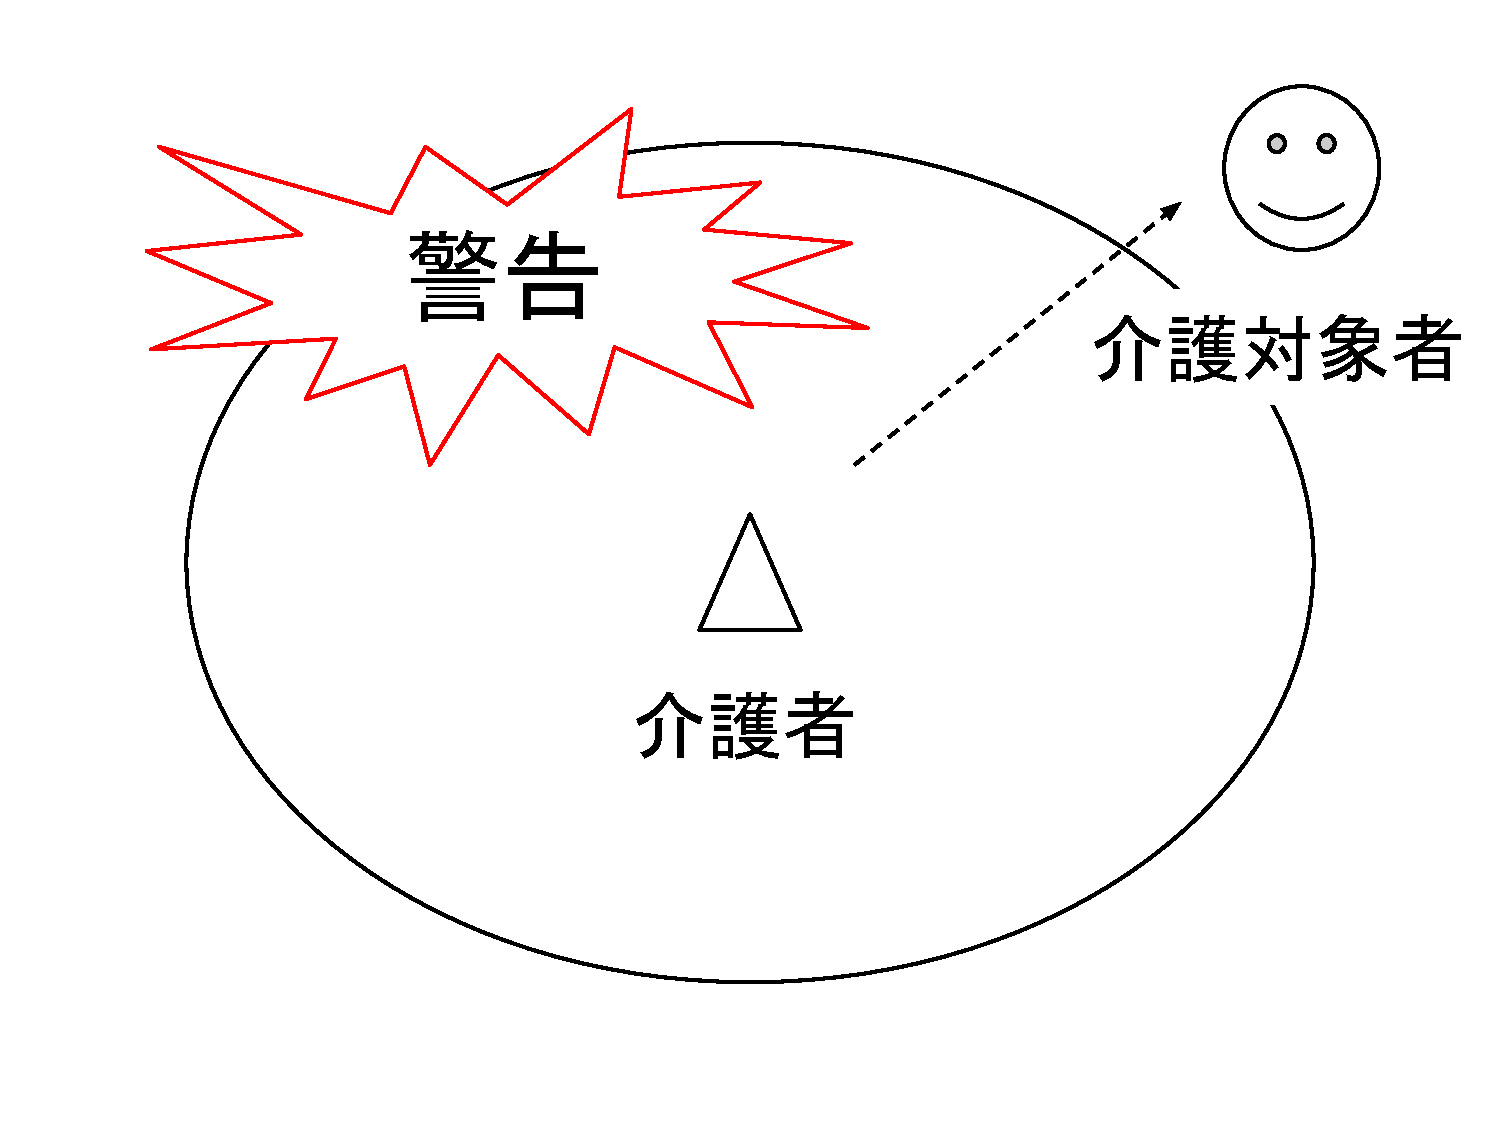
\includegraphics[width=10cm]{fig/deviation.pdf}
\caption{見守りエリアからの逸脱管理}
\end{figure}

\section{ビーコン情報の共有}
受信用スマートフォンが複数ある場合は,スマートフォン同士で発信機の情報を共有し,見守りエリアを拡大させる.
自らの見守りエリアから逸脱した発信機が,他のスマートフォンで検知されていれば見守りは成功していると判断で
きる.
スマートフォン同士で共有する発信機の情報は,

\begin{itemize}
\item タイムスタンプ
\item 各自の見守りエリアにある発信機ID
\item 見守りエリアから逸脱した発信機ID
\end{itemize}

以上の三つである.これらの情報を共有することで,同じアドホックネットワーク内にある他のスマートフォンが検知している発信機を知ることができ,見守りエリアを拡大することができる.

\begin{figure}[htbp]
\centering
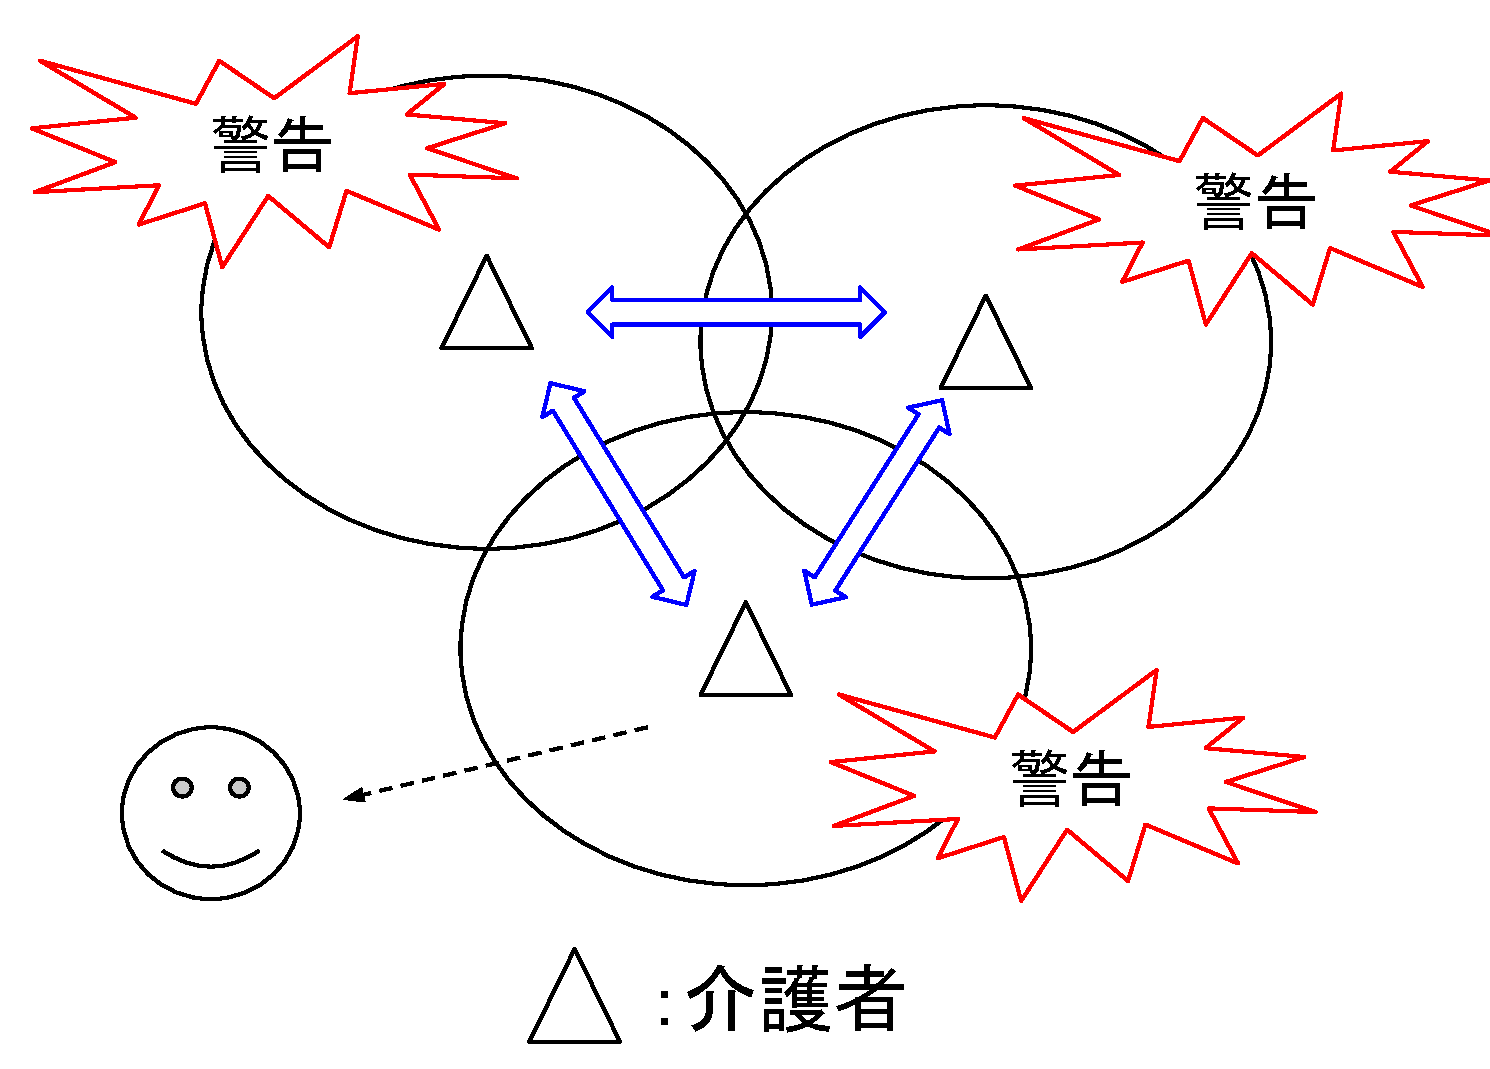
\includegraphics[width=10cm]{fig/share.pdf}
\caption{ビーコン情報の共有}
\end{figure}
